\section{Results}

The author permitted to see the grand academy of Lagado.  The academy largely described.  The arts wherein the professors employ themselves.

\begin{figure}
\begin{subfigure}{.5\linewidth}
\centering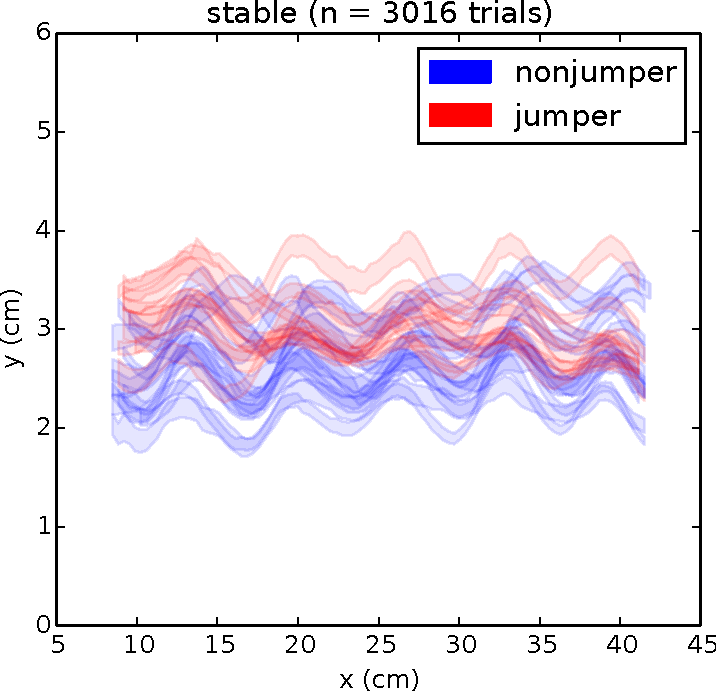
\includegraphics[width=\columnwidth]{chapters/figuresChBehaviour/noseTrajectoryStable}
\label{fig:noseTrajectoryStable}
\end{subfigure}%
\begin{subfigure}{.5\linewidth}
\centering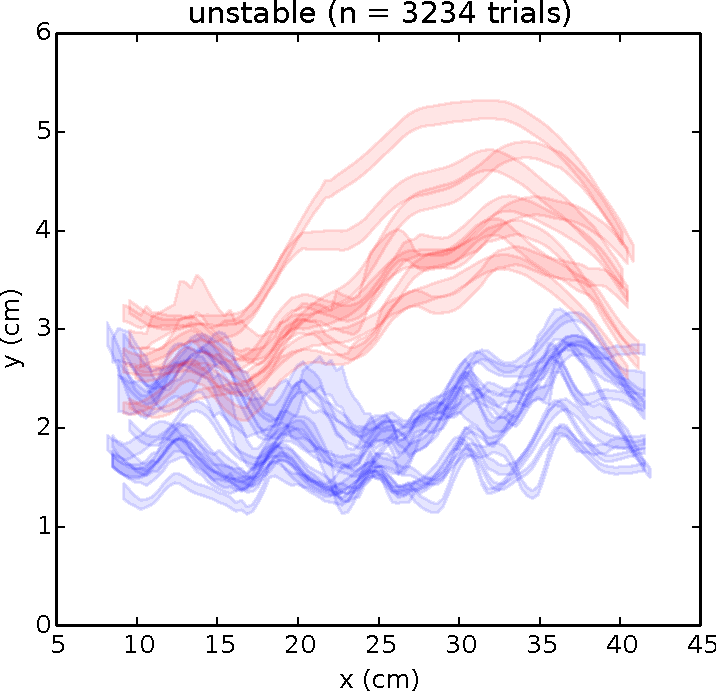
\includegraphics[width=\columnwidth]{chapters/figuresChBehaviour/noseTrajectoryUnstable}
\label{fig:noseTrajectoryUnstable}
\end{subfigure}\\[1ex]
\begin{subfigure}{\linewidth}
\centering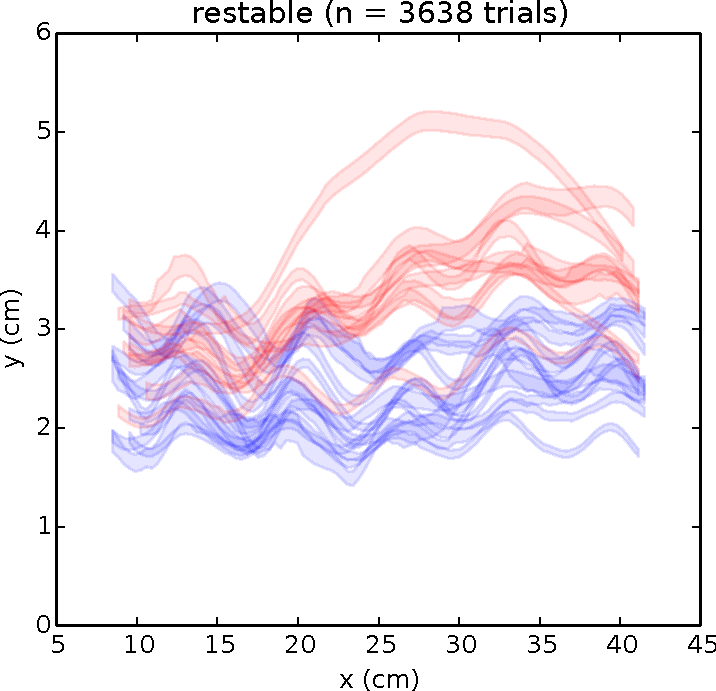
\includegraphics[width=.5\columnwidth]{chapters/figuresChBehaviour/noseTrajectoryRestable}
\label{fig:noseTrajectoryRestable}
\end{subfigure}
\caption{\textbf{Average nose trajectories when crossing the obstacles under different conditions of the shuttling protocol.} Each line represents the average nose trajectory for each individual animal. Line thickness indicates standard error of the mean. Leftward trials were mirrored so that progression is always from left to right. Classification of an animal into jumper or non-jumper was done on the basis of their trajectory in the \emph{unstable} condition and retained throughout.}
\label{fig:noseTrajectory}
\end{figure}

\begin{figure}
\begin{center}
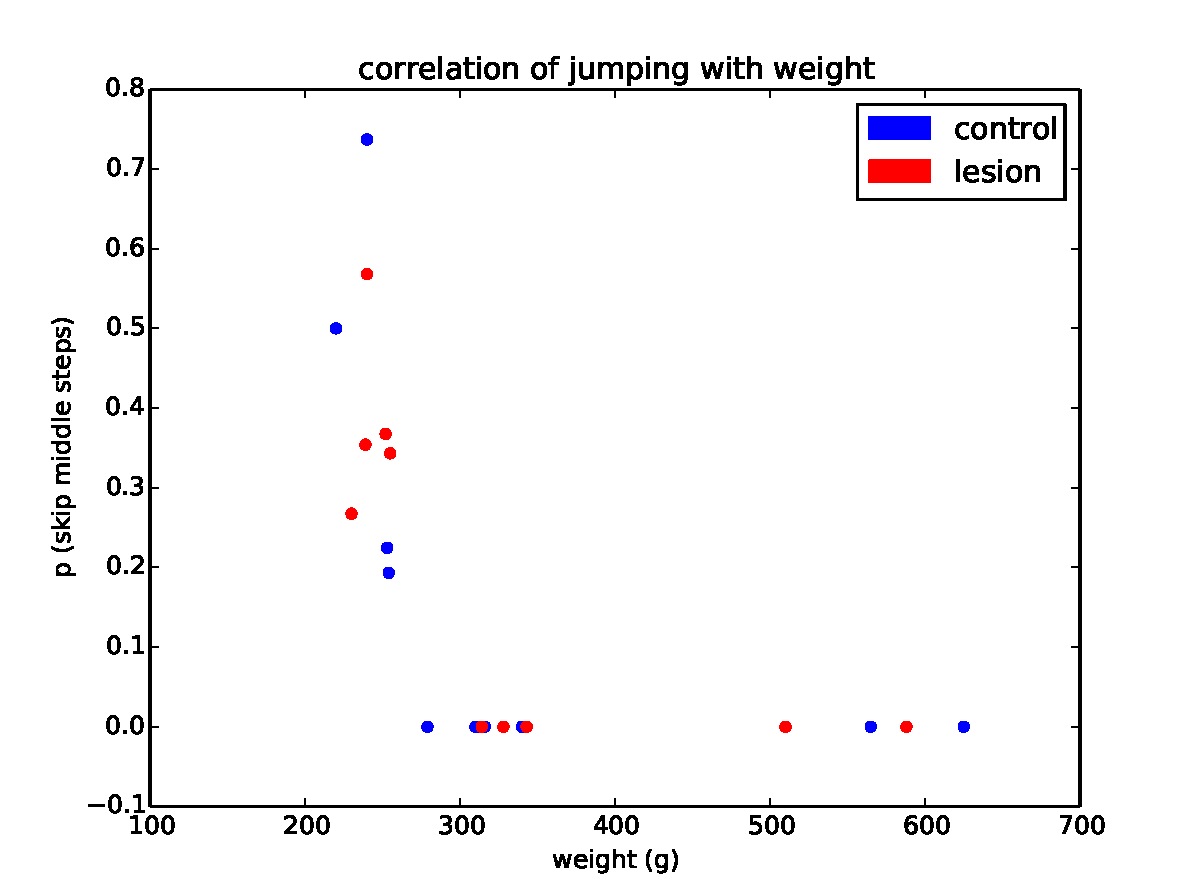
\includegraphics[width=\columnwidth]{chapters/figuresChBehaviour/correlationJumperWeight}
\end{center}
\vspace{-5mm}
\caption{\textbf{Probability of skipping both middle steps in unstable sessions correlated with body weight.} Each dot represents an individual animal. Body weights were taken from the first habituation session before starting the water deprivation protocol. A trial was marked as skipped if neither of the regions of interest in the middle steps were activated by any body part of the animal in that trial.}
\label{fig:correlationJumperWeight}
\end{figure}

\begin{figure}
\begin{subfigure}{.3\linewidth}
\centering\scalebox{0.5}{\inputpgf{chapters/figuresChBehaviour}{averagePostureCa.pgf}}
\label{fig:averagePostureCa}
\end{subfigure}%
\begin{subfigure}{.3\linewidth}
\centering\scalebox{0.5}{\inputpgf{chapters/figuresChBehaviour}{averagePostureCb.pgf}}
\label{fig:averagePostureCb}
\end{subfigure}%
\begin{subfigure}{.3\linewidth}
\centering\scalebox{0.5}{\inputpgf{chapters/figuresChBehaviour}{averagePostureCc.pgf}}
\label{fig:averagePostureCc}
\end{subfigure}
\vspace{-5mm}\\
\begin{subfigure}{.3\linewidth}
\centering\scalebox{0.5}{\inputpgf{chapters/figuresChBehaviour}{averagePostureCd.pgf}}
\label{fig:averagePostureCd}
\end{subfigure}%
\begin{subfigure}{.3\linewidth}
\centering\scalebox{0.5}{\inputpgf{chapters/figuresChBehaviour}{averagePostureCe.pgf}}
\label{fig:averagePostureCe}
\end{subfigure}%
\begin{subfigure}{.3\linewidth}
\centering\scalebox{0.5}{\inputpgf{chapters/figuresChBehaviour}{averagePostureCg.pgf}}
\label{fig:averagePostureCf}
\end{subfigure}
\vspace{-5mm}\\
\begin{subfigure}{.3\linewidth}
\centering\scalebox{0.5}{\inputpgf{chapters/figuresChBehaviour}{averagePostureCk.pgf}}
\label{fig:averagePostureCd}
\end{subfigure}%
\begin{subfigure}{.3\linewidth}
\centering\scalebox{0.5}{\inputpgf{chapters/figuresChBehaviour}{averagePostureLb.pgf}}
\label{fig:averagePostureCe}
\end{subfigure}%
\begin{subfigure}{.3\linewidth}
\centering\scalebox{0.5}{\inputpgf{chapters/figuresChBehaviour}{averagePostureLd.pgf}}
\label{fig:averagePostureCf}
\end{subfigure}
\vspace{-5mm}\\
\begin{subfigure}{.3\linewidth}
\centering\scalebox{0.5}{\inputpgf{chapters/figuresChBehaviour}{averagePostureLe.pgf}}
\label{fig:averagePostureCd}
\end{subfigure}%
\begin{subfigure}{.3\linewidth}
\centering\scalebox{0.5}{\inputpgf{chapters/figuresChBehaviour}{averagePostureLg.pgf}}
\label{fig:averagePostureCe}
\end{subfigure}%
\begin{subfigure}{.3\linewidth}
\centering\scalebox{0.5}{\inputpgf{chapters/figuresChBehaviour}{averagePostureLk.pgf}}
\label{fig:averagePostureCf}
\end{subfigure}
\vspace{-5mm}
\caption{\textbf{Average posture on approach to the manipulated step under stable (green) and unstable (red) conditions.}}
\label{fig:averagePosture}
\end{figure}

\begin{figure}
\begin{subfigure}{.3\linewidth}
\centering\scalebox{0.5}{\inputpgf{chapters/figuresChBehaviour}{averagePostureCh.pgf}}
\label{fig:averagePostureCa}
\end{subfigure}%
\begin{subfigure}{.3\linewidth}
\centering\scalebox{0.5}{\inputpgf{chapters/figuresChBehaviour}{averagePostureCj.pgf}}
\label{fig:averagePostureCb}
\end{subfigure}%
\begin{subfigure}{.3\linewidth}
\centering\scalebox{0.5}{\inputpgf{chapters/figuresChBehaviour}{averagePostureCf.pgf}}
\label{fig:averagePostureCc}
\end{subfigure}
\vspace{-5mm}\\
\begin{subfigure}{.3\linewidth}
\centering\scalebox{0.5}{\inputpgf{chapters/figuresChBehaviour}{averagePostureCi.pgf}}
\label{fig:averagePostureCd}
\end{subfigure}%
\begin{subfigure}{.3\linewidth}
\centering\scalebox{0.5}{\inputpgf{chapters/figuresChBehaviour}{averagePostureLc.pgf}}
\label{fig:averagePostureCe}
\end{subfigure}%
\begin{subfigure}{.3\linewidth}
\centering\scalebox{0.5}{\inputpgf{chapters/figuresChBehaviour}{averagePostureLh.pgf}}
\label{fig:averagePostureCf}
\end{subfigure}
\vspace{-5mm}\\
\begin{subfigure}{.3\linewidth}
\centering\scalebox{0.5}{\inputpgf{chapters/figuresChBehaviour}{averagePostureLj.pgf}}
\label{fig:averagePostureCd}
\end{subfigure}%
\begin{subfigure}{.3\linewidth}
\centering\scalebox{0.5}{\inputpgf{chapters/figuresChBehaviour}{averagePostureLf.pgf}}
\label{fig:averagePostureCe}
\end{subfigure}%
\begin{subfigure}{.3\linewidth}
\centering\scalebox{0.5}{\inputpgf{chapters/figuresChBehaviour}{averagePostureLi.pgf}}
\label{fig:averagePostureCf}
\end{subfigure}
\vspace{-5mm}
\caption{\textbf{Average posture on approach to the manipulated step for the jumper group under stable (green) and unstable (red) conditions.}}
\label{fig:averagePosture}
\end{figure}